\PassOptionsToPackage{utf8}{inputenc}
\documentclass{bioinfo}
\copyrightyear{2015} \pubyear{2015}

\access{Advance Access Publication Date: Day Month Year}
\appnotes{Manuscript Category}

\begin{document}
\firstpage{1}

\subtitle{Subject Section}

\title[PCRedux]{Automatic Classification of Quantitative PCR Amplification Curves}
\author[Burdukiewicz \textit{et~al}.]{
Micha\l{} Burdukiewicz\,$^{\text{\sfb 1}}$,
Andrej-Nikolai Spiess\,$^{\text{\sfb 2}}$,
Matthew N. McCall\,$^{\text{\sfb 3}}$,
Stefan R\"{o}diger\,$^{\text{\sfb 4},*}$
}
\address{
$^{\text{\sf 1}}$Faculty of Mathematics and Information Science, University of 
Wroc\l{}aw, Wroc\l{}aw, Poland,
$^{\text{\sf 2}}$University Medical Center Hamburg-Eppendorf, Hamburg, Germany, 
$^{\text{\sf 3}}$University of Rochester Medical Center,
$^{\text{\sf 4}}$Institute of Biotechnology, Brandenburg University of Technology 
Cottbus~--~Senftenberg, Senftenberg, Germany.
}
\corresp{$^\ast$To whom correspondence should be addressed.}

\history{Received on XXXXX; revised on XXXXX; accepted on XXXXX}

\editor{Associate Editor: XXXXXXX}

\abstract{\textbf{Motivation:} There are numerous examples of data with a sigmoid ('S'-shaped) curves in data science. One example is amplification curve data from quantitative Polymerase chain reactions (qPCR). The qPCR is an indispensable technology in human diagnostics and forensics. From an amplification curve quantitative information can be determined which can be used to assess diseases.\\
\textbf{Results:} The web server uses the machine learning mlr package as interface to a large number of classification and regression techniques. The PCRedux can be used for the extraction of features and for machine learning on amplification curves. The PCRedux package is an add-on package (MIT license) for open source statistical computing language and environment R. The PCRedux package contains functions and classified amplification curves for machine learning and statistical analysis. In addition, the PCRedux package contains extensive labelled data sets of amplification curves from various qPCR devices and detection chemistries. The amplification curves were classified (negative, positive) by a human. For curve shape based classification, the tReem() funftion was developed. To analyze the amplification curves methods such as change-point analysis, regression analysis, autocorrelation analysis and model fitting have been integrated. The pcrfit\_single() function calculate more than 45 features from the amplification curves. This is useful for creating models and predicting classes (e. g. negative, positive).\\
\textbf{Availability:} The PCRedux web server for the analysis of amplification curves using the PCRedux package is available from \url{http://www.smorfland.uni.wroc.pl/shiny/predPCR/}.\\
\textbf{Contact:} \href{stefan.roediger@b-tu.de}{stefan.roediger@b-tu.de}\\
\textbf{Supplementary information:} Supplementary data are available at \textit{Bioinformatics}
online.}

\maketitle

\section{Introduction}

Quantitative polymerase chain reaction (qPCR) is a widely used bioanalytical method in forensics,
human diagnostics and life sciences. With this method nucleic acids are detected and quantified.
In qPCRs, the enzymatic amplification of the target DNA (amplicon) is monitored in real-time
by fluorescent reporter molecules marking the synthesized PCR products cycle by cycle. The
measured fluorescence is proportional to the amplicon amount \citep{pabinger_2014}.

For diagnostic and forensic applications in particular, the question arises as to whether an amplification reaction is negative or positive. Until now, such classification was usually performed manually or on the
basis of fixed threshold values. However, this approach is error-prone if inadequate thresholds are
used or the user performs the classification subjectively based on his experience. Therefore, the
classifications of the same sample may not be identical for different users. In forensic applications
in particular, such errors are problematic because they can lead to an erroneous judgement.


The relevance of high-throughput qPCR

Showcase than qPCR is relevant as a complementary stuff to NGS.

What are qPCR features? A way to represent qPCR curve as a single (most often numerical) value

We based our predictive algorithm on these features, to make predictions understandable for experimentalists

A review of the literature and discussion with peers revealed that there is no open source software
package to calculate predictors from quantitative PCR amplification curves for machine learning
applications. A predictor is a quantifiable informative property of an amplification curve. In
particular, there is no information available about predictors that can be used from amplification
curves apart from measures that describe quantification points, amplification efficiencies and
signal levels. Although several amplification curve data sets are available, no curated labeled
data sets labels are described in the literature or repositories.
\begin{methods}
\section{Methods}

Datasets

Features, correlation matrix of features

Why we sticked to the grid search of the most optimal parameters

Present three the most informative features.

\end{methods}


\section{Results and discussion}

\begin{figure}
\centerline{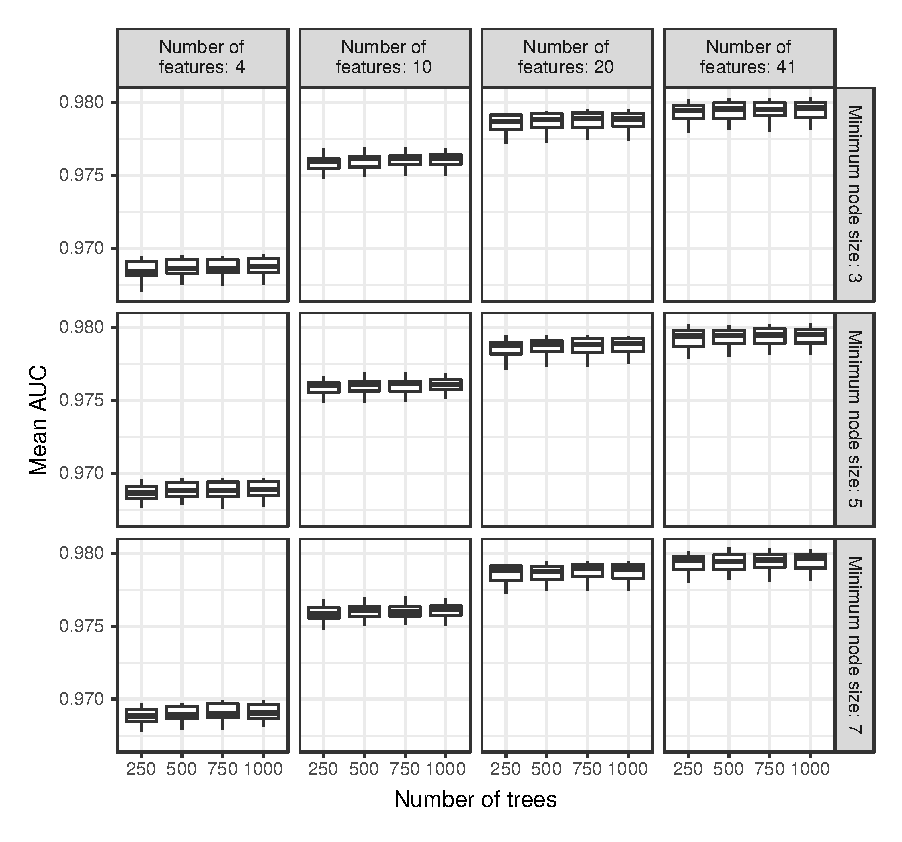
\includegraphics{figures/AUC.eps}}
\caption{Mean AUC of qPCR curve classification.}\label{fig:AUC}
\end{figure}

PCRedux is an open source software package (MIT license) for the statistical computing language
R. Data with sigmoid curves are common in bioanalytical methods, such as in the widely used
real-time PCR (qPCR), applied in human diagnostics, life sciences and forensics (Martins et al.
2015; Sauer et al. 2016). qPCR amplification curves are an example for sigmoid shaped curves,
for which PCRedux contains functions to calculate predictors and classify data sets for machine
learning applications.

In addition to the determination of quantification points, the classification of amplification curves
is necessary. For example, a diagnostician is interested in whether a sample is positive or negative.
In research using high-throughput screening methods, it is important to classify large data sets
quickly and cost-effectively. It is important to bear in mind that in manual classification, the
classification result is influenced by the subjective perception of the experimenter and that it is
comparatively time-consuming.

With this software, predictors (features) of amplification curves can be calculated automatically. A
predictor is a quantifiable informative property of an amplification curve. An achievement of
this study is the extensive portfolio of statistical algorithms for the calculation of predictors.
Accordingly, the statistical analysis of amplification curves is presented in detail. Furthermore,
the work deals with elements of software engineering (e.g. continuous integration, unit testing),
which were applied within the research work. The work also shows how predictors can be used
in tests and logical combinations to perform machine-based classifications.
All scientific work depends on the data, with open data in particular being regarded as a
cornerstone of science. Since no data sets of classified amplification curves were available, the
work also deals with the aggregation, management and distribution of classified qPCR data
sets. Manual classification of amplification curves is time-consuming and error-prone, especially
for large data sets. To improve this, auxiliary tools have been developed. A new approach for
curve-shape based group classification was found.
All findings were implemented in the PCRedux software for the statistical
language R.

Discuss three the most important features here.

\section*{Acknowledgements}

Grateful thanks belong to the \textbf{R} community.\vspace*{-12pt}

\section*{Funding}

This work was funded by the Federal Ministry of Education and Research (BMBF) InnoProfile-Transfer-Projekt 03 IPT 611X.\vspace*{-12pt}

\bibliographystyle{natbib}
%\bibliographystyle{achemnat}
%\bibliographystyle{plainnat}
%\bibliographystyle{abbrv}
%\bibliographystyle{bioinformatics}
%
%\bibliographystyle{plain}
%
\bibliography{literature}


% \begin{thebibliography}{}

% \bibitem[Bofelli {\it et~al}., 2000]{Boffelli03}
% Bofelli,F., Name2, Name3 (2003) Article title, {\it Journal Name}, {\bf 199}, 133-154.

% \bibitem[Bag {\it et~al}., 2001]{Bag01}
% Bag,M., Name2, Name3 (2001) Article title, {\it Journal Name}, {\bf 99}, 33-54.

% \bibitem[Yoo \textit{et~al}., 2003]{Yoo03}
% Yoo,M.S. \textit{et~al}. (2003) Oxidative stress regulated genes
% in nigral dopaminergic neurnol cell: correlation with the known
% pathology in Parkinson's disease. \textit{Brain Res. Mol. Brain
% Res.}, \textbf{110}(Suppl. 1), 76--84.

% \bibitem[Lehmann, 1986]{Leh86}
% Lehmann,E.L. (1986) Chapter title. \textit{Book Title}. Vol.~1, 2nd edn. Springer-Verlag, New York.

% \bibitem[Crenshaw and Jones, 2003]{Cre03}
% Crenshaw, B.,III, and Jones, W.B.,Jr (2003) The future of clinical
% cancer management: one tumor, one chip. \textit{Bioinformatics},
% doi:10.1093/bioinformatics/btn000.

% \bibitem[Auhtor \textit{et~al}. (2000)]{Aut00}
% Auhtor,A.B. \textit{et~al}. (2000) Chapter title. In Smith, A.C.
% (ed.), \textit{Book Title}, 2nd edn. Publisher, Location, Vol. 1, pp.
% ???--???.

% \bibitem[Bardet, 1920]{Bar20}
% Bardet, G. (1920) Sur un syndrome d'obesite infantile avec
% polydactylie et retinite pigmentaire (contribution a l'etude des
% formes cliniques de l'obesite hypophysaire). PhD Thesis, name of
% institution, Paris, France.

% \end{thebibliography}
\end{document}
